% Template for Cogsci submission with R Markdown

% Stuff changed from original Markdown PLOS Template
\documentclass[10pt, letterpaper]{article}

\usepackage{cogsci}
\usepackage{pslatex}
\usepackage{float}
\usepackage{caption}

% amsmath package, useful for mathematical formulas
\usepackage{amsmath}

% amssymb package, useful for mathematical symbols
\usepackage{amssymb}

% hyperref package, useful for hyperlinks
\usepackage{hyperref}

% graphicx package, useful for including eps and pdf graphics
% include graphics with the command \includegraphics
\usepackage{graphicx}

% Sweave(-like)
\usepackage{fancyvrb}
\DefineVerbatimEnvironment{Sinput}{Verbatim}{fontshape=sl}
\DefineVerbatimEnvironment{Soutput}{Verbatim}{}
\DefineVerbatimEnvironment{Scode}{Verbatim}{fontshape=sl}
\newenvironment{Schunk}{}{}
\DefineVerbatimEnvironment{Code}{Verbatim}{}
\DefineVerbatimEnvironment{CodeInput}{Verbatim}{fontshape=sl}
\DefineVerbatimEnvironment{CodeOutput}{Verbatim}{}
\newenvironment{CodeChunk}{}{}

% cite package, to clean up citations in the main text. Do not remove.
\usepackage{apacite}

% KM added 1/4/18 to allow control of blind submission


\usepackage{color}

% Use doublespacing - comment out for single spacing
%\usepackage{setspace}
%\doublespacing


% % Text layout
% \topmargin 0.0cm
% \oddsidemargin 0.5cm
% \evensidemargin 0.5cm
% \textwidth 16cm
% \textheight 21cm

\title{English Negative Constructions and Communicative Functions in Child
Language}


\author{{\large \bf Zoey Liu (ying.liu.5@bc.edu)} \\ Department of Computer Science \\ Boston College \AND {\large \bf Masoud Jasbi (jasbi@ucdavis.edu)} \\ Department of Linguistics \\ University of California, Davis}


\begin{document}

\maketitle

\begin{abstract}
How does negation emerge in early conceptual and linguistic development?
Previous research has hypothesized that negation develops to express
communicative functions such as rejection, non-existence, or
prohibition. However, findings from prior work have mostly relied on
manual annotations to identify negative utterances of different
functions, leading the number of children as well as the size of the
data sets analyzed to be relatively small. This study considers specific
syntactic constructions combined with negative morphemes (\emph{no},
\emph{not}, \emph{n't}) in English as expressions of different
communicative functions for negation. Leveraging larges-scale corpora of
child-parent interactions along with computational tools, we examine the
developmental trajectories of seven different functions and their
corresponding negative constructions. Our analyses demonstrate a
gradually increasing usage of negation in all functions between the ages
of 24 - 36 months; yet there are notable differences in the earlier
developmental stages of negation depending on the particular function
investigated.

\textbf{Keywords:}
negation; syntax construction; communicative function; development;
child language.
\end{abstract}

\hypertarget{introduction}{%
\section{Introduction}\label{introduction}}

Negation is an abstract concept crucial to everyday communication. It
can help a coffee shop divide its menu into ``coffee'' and ``not
coffee'' sections, with the ``not coffee'' section bringing together
diverse items with no common label. It can inform us to regulate each
others' actions in a sign like ``no mask, no entry''. It can also
communicate our deepest wants and dislikes as in ``I don't like
Mondays''. But how does the abstract concept of negation emerge in the
human mind? What are the specific communicative functions that negation
combines with in early language development?

Starting a century and a half ago, Darwin (1872) thought that negation
has roots in the expression of human emotions and desires. He
hypothesized the earliest manifestation of negation and affirmation in
infants is when they refuse food from parents, by withdrawing their
heads laterally, or when they accept the food, by inclining their heads
forward. He suggested that head shaking and nodding as common gestures
for negation and affirmation have developed from this early habit.
Similarly, many researchers studying early functions of negative
morphemes like \emph{no} proposed that children use them to ``reject''
or ``refuse'' (Bloom, 1970; Choi, 1988; Pea, 1978). For example, when
they are asked ``do you want juice?'', they may say ``no'', ``not want
it'', or ``don't like it''. Pea (1978) proposed this negation function
is the first to emerge in children's early speech.

Bloom (1970) argued that the use of negation to expresses
``non-existence'' emerges before rejection or refusal. For example, when
an object that children expect to be present is not present, children
may say: ``no window'', ``no fish in the bathroom'', or ``I do not have
underpants''. Two close concepts to non-existence are ``disappearance''
and ``non-occurrence'' (Pea, 1978; Villiers \& Villiers, 1979).
Disappearance refers to situations where an object disappears and
children use negation to express it (e.g.~``no food. all gone'' or ``no
more noise''). Non-occurrence refers to cases when an expected action or
event does not occur as in ``not working'' or ``doggie not barking''.
Some researchers referred to these cases as ``failures'' and included
examples like ``no fit in da box'' or ``it don't fit''
(Cameron-Faulkner, Lieven, \& Theakston, 2007; Choi, 1988).
Non-existence can also be expressed by negation of locative
prepositional phrases (e.g.~``no in there'' or ``daddy was not on the
phone''). While rejection was hypothesized to interact with human
emotions and desires, non-existence (broadly construed to include
``disappearance'' and ``non-occurrence'') likely interacts with human
perception. Choi (1988) proposed that children's early linguistic
negation is used to express both rejection and non-existence.

Additionally, Choi (1988) introduced ``prohibition'' and suggested that
it emerges as early as rejection and non-existence. In cases of
prohibition, children use negation to stop others from performing
actions; for example ``don't go'' or ``do not spill milk''. A special
case of prohibition is ``self-prohibition''. For example, a child may
approach prohibited food but immediately say ``no, don't eat'' to stop
themselves. A function similar to prohibition is ``inability''
(e.g.~\emph{I can't reach} / \emph{I cannot zip it}), in that both
involve conceptualizing actions and negating them, possibly interacting
with early development of motor control. Choi (1988) suggested that
expression of inability emerges after the first phase, namely
non-existence, rejection, and prohibition.

``Denial'' is another function of negation that is argued to be late in
development. Bloom (1970) defined it as asserting that ``an actual or
supposed predication was not the case'', for example ``It's not sharp''.
Later researchers formulated it as ``truth-functional negation'' because
it is used to negate the truth of a proposition (Cameron-Faulkner et
al., 2007; Pea, 1978). However, this definition depends on the assumed
logical system and its assumptions on what type of propositions receive
truth values. A particular sub-function of denial is ``labeling'', which
is realized as the negation of nominal or adjectival predicates such as
``this is not a bunny'' or ``not red''. These utterances are often used
to introduce new linguistic labels by parents and in turn may facilitate
word learning (Clark, 2010). Conversely, labeling and word learning may
aid the development of abstract negation.

Despite considerable research on early functions of negation, their
developmental trajectories in children's productions have remained
unclear. Different studies have claimed different order of acquisition
(Pea, 1978). In a recent study, Nordmeyer \& Frank (2018) looked at the
speech of five children in the Providence corpus (Demuth, Culbertson, \&
Alter, 2006) and found a great deal of individual differences in how
early a negative function is attested. This is partly because previous
studies have had to rely on human annotation and identification of
functions from corpus data, a time-consuming and difficult process that
has limited previous studies to a handful of children and a relatively
small sample of their speech.

Our study addresses this question by using syntactic constructions as a
proxy for communicative functions. We used a large collection of child
speech corpora in English (MacWhinney, 2000) with part of speech tags
and syntactic dependency relations. We automatically selected
constructions that conveyed the functions discussed in prior research
and asked: (1) how early do these constructions emerge in children's
speech and what's their trajectory? (2) within the same communicative
function, does the developmental trajectory differ depending on
particular lexical items that negation modifies (e.g.~\emph{like} or
\emph{want} for rejection)? (3) taking all functions into account, do
they share similar developmental characteristics, or would there be
function-specific differences?

Q1: How does the developmental trajectory of each communicative function
look like? Q2: How do the developmental trajectories of different
communicative functions vary?

Mention in Introduction (and/or connect in Experiments section after
things are finalized): these negative constructions do not cover
everything that negation could be combined with, and that the negative
constructions are not the only ways of conveying different communicative
functions

\begin{table*}[h]
\small
\centering
\begin{tabular}{rrr}
  \hline
 \textbf{Function} & \textbf{Linguistic Composition} & \textbf{Examples} \\
  \hline
Rejection & with \textit{like} or \textit{want} & \textit{I not like it}, \textit{not want it}  \\
Non-existence & expletives & \textit{there is no soup} \\
Prohibition & with imperative subjectless \textit{do} & \textit{do not spill milk} \\
Inability & with modal \textit{can} & \textit{I cannot zip it} \\
Labeling & modifying nominal or adjectival predicatives & \textit{that's not a crocodile}; \textit{it's no interesting} \\
Epistemic negation & with \textit{know}, \textit{think}, \textit{remember}  & \textit{I not know} \\
Possession & with \textit{have}; or possesive pronouns & \textit{not have the toy}; \textit{not mine} \\
   \hline
\end{tabular}
\caption{Communicative functions of negation in early child language of English.}
\end{table*}

\hypertarget{experiments}{%
\section{Experiments}\label{experiments}}

\hypertarget{data-and-preprocessing}{%
\subsection{Data and preprocessing}\label{data-and-preprocessing}}

For developmental production data of child language in English, we
turned to the CHILDES database (MacWhinney,
2000).\footnote{Code and data are in quarantine at \url{https://github.com/zoeyliu18/Negative_Constructions.}}.
We focused on speech produced by children with typical development
within the age range of 12 - 72 months, specifically at the
single-sentence level (as opposed to the discourse level). Utterances of
child and parent speech were extracted via the childes-db (Sanchez et
al., 2019) interface using the programming language R. Negative
structures were then identified based on whether a structure contains
any of the three negative morphemes: \emph{no}, \emph{not} and
\emph{n't}. Since the matters of interest here are syntactic structures
\emph{combined} with negation, cases consisting of one negative morpheme
(e.g.~\emph{no}!) or repetition of negative morphemes (e.g.~\emph{no no
no}!) were not considered.

In order to conduct analysis of negative syntactic constructions and the
particular communicative functions that they serve, we need to first
obtain (morpho)syntactic representations of child and parent speech. To
do that, we opted for the dependency grammar framework (Tesnière, 1959);
the syntactic dependency relations of all negative utterances were
automatically derived with DiaParser (Attardi, Sartiano, \& Yu, n.d.), a
dependency parsing system that has been demonstrated to achieve
excellent performance for English. And to further facilitate
identifications of negative constructions, we also utilized the
available part-of-speech (POS) information initially provided by CHILDES
(Sagae, Davis, Lavie, MacWhinney, \& Wintner, 2010) when necessary.

Besides the functions of rejection, non-existence, prohibition,
inability and labeling (the sub-function of denial), we expanded with
two other functions: epistemic negation (Choi, 1988) and possession (see
Table 1). For each function, using our parsed data set, we characterized
the syntactic features of the negative constructions associated with
that function. Based on these features, negative utterances were
automatically extracted in a rule-based fashion with the help of POS
information and syntactic dependencies.

\hypertarget{measures}{%
\subsection{Measures}\label{measures}}

As indexes of the developmental trajectory for negative constructions
and their communicative functions in child speech, we measured the
following two metrics at each given age of the children. The first one
is the \emph{ratio} of negative utterances. For instance, the number of
utterances produced by children at the age of 30 months (not just all
negative constructions at this age) is 52,491 in total. Among these
utterances, negative structures that have the function fo inability
occur for 141 times; the ratio for this communicative function at 30
months is then calculated as 141 / 52,491 = 0.003.

Given the noisy nature of child production data in general, and the
facts that there are different numbers of utterances and children at
each age, another measure that we utilized is \emph{moving ratio},
borrowed from the model of moving average in analyses of time series
data (Wei, 2006). For a communicative function, the goal of the moving
ratio is still to reflect the production of the negative utterances at
the given age; meanwhile it takes into account the previous production
of all negative constructions of the same function before the specified
age. This would allow us to have a more balanced look at individual
developmental stage (e.g.~age) of a communicative function, in relation
to its development patterns thus far.

The computation of the moving ratio is as follows. For instance, given
that the number of negative utterances that express inability in child
speech is 141 at the age of 30 months, we: (1) count the total number of
negative constructions with the same function produced by children
\emph{at and before} 30 months old (682); (2) compute the total number
of utterances (419,949) within the same age range; (3) divide the number
of (1) by that of (2) (682 / 419,949 = 0.002).

While our focus is negative utterances in child production, we used
parents' speech as comparative references. Therefore for every
communicative function, the same two ratio measures were calculated for
parent speech in a similar fashion. Our plots accordingly contrast the
ratio / moving ratio of different negative constructions between
children's and parents' production at corresponding ages of the
children.

In what follows, we describe in detail the results of each communicative
function and their negative constructions. While we computed both ratio
and moving ratio for every function, our analyses mainly rely on the
latter.

\hypertarget{communicative-functions-of-negative-constructions}{%
\subsection{Communicative functions of negative
constructions}\label{communicative-functions-of-negative-constructions}}

\hypertarget{rejection}{%
\subsubsection{Rejection}\label{rejection}}

For the function of rejection, we examined cases where the lemma of the
head verb of the phrase is either \emph{like} or \emph{want}, and the
head verb is modified by one of the three negative morphemes. Each of
the utterances either takes a subject or has no subject at all. And the
existence of a subject was determined via searching for a word in the
utterance that has the \emph{nsubj} dependency relation with the head
verb.

Additionally, other than expressions that the speakers used to describe
their own emotion, with (e.g.~(1)) or without (e.g.~(2)) an auxiliary
verb, we also included cases that express rhetorical inquiries of
emotions from one interlocutor addressed to another (e.g.~(3)) as well
as instances where the speaker is describing the emotion of somebody
else (e.g.~(4)). Overall our data extraction resulted in a total of
17,436 negative utterances (child: 7,395; parent: 10,041).

~ (1) \emph{I no like sea}

~ (2) \emph{don't wanna go}

~ (3) \emph{don't you wanna try it}

~ (4) \emph{Sarah doesn't like that either}

\begin{figure*}[h]

\begin{CodeChunk}


\begin{center}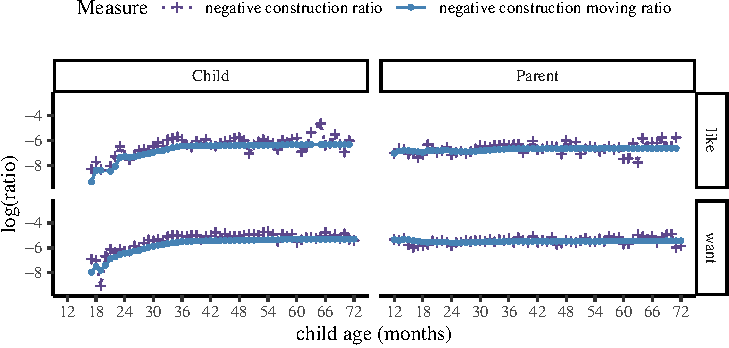
\includegraphics{figs/emotion-1} \end{center}

\end{CodeChunk}
\caption[This image spans both columns]{Rejection.}\label{fig:rejection}
\end{figure*}

As presented in Figure 1, within the context of the corpus data that we
analyzed, the overall pattern for children's usage of negative morphemes
for rejection is comparable regardless of the particular head verb.
Comparing child and parent speech, it seems that children's production
of rejection is gradually increasing between the age of 19 to 36 months.
And the production moving ratio in child speech appears to be more
comparable to that of parent speech after 32-34 months.

\hypertarget{non-existence}{%
\subsubsection{Non-existence}\label{non-existence}}

For the function of non-existence, in order to not confuse with the
function of labeling (see below), we extracted utterances that have
expletives marked by \emph{there} (e.g.~(5) and (6)), and that the
predicate modified by the negative morphemes is a nominal phrase (headed
by either nouns or pronouns). This led to a total of 1,611 negative
utterances (child: 406; parent: 1,205).

~ (5) \emph{there's no (more) water}

~ (6) \emph{there isn't it}

In child speech, the production of negative constructions to express
non-existence is gradually increasing from 27 to 36 months (Figure 2),
which is by contrast later than that for the communicative function of
rejection presented in Figure 1. This is observation does not seem to
align with Bloom (1970), which initially proposed that the development
of non-existence is earlier than that of rejection. On the other hand,
children's production moving ratio gradually approaches that in parent
speech at 36-38 months.

Notice that there appears to be fluctuations of moving ratios between
the age of 19 and 27 months regarding child production. A closer
inspection of the data reveals that within that age range, the frequency
of negative utterances at most ages is either one or zero. Therefore
while the number of total utterances increases along the developmental
trajectory, the moving ratio for negative utterances actually decreases.

\begin{figure*}[h]

\begin{CodeChunk}


\begin{center}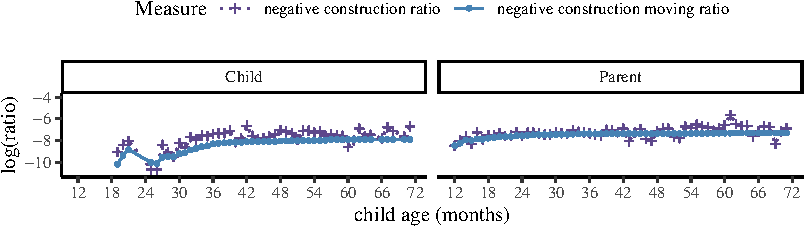
\includegraphics{figs/existence-1} \end{center}

\end{CodeChunk}
\caption[This image spans both columns]{Non-existence.}\label{fig:non-existence}
\end{figure*}

\hypertarget{prohibition}{%
\subsubsection{Prohibition}\label{prohibition}}

For constructions that articulate the function of prohibition, we
focused on cases that are annotated as imperatives from the initial
CHILDES annotations. These utterances do not take any subject; the
negative morphemes are combined with the auxiliary verb \emph{do}
(\emph{do}, \emph{does}, \emph{did}) and they together modify the head
verbs of the sentences. In order to not overlap with rejection,
non-existence, epistemic negation and possession (see below), our search
excluded cases where the head verb has any of the following lemma forms:
\emph{like}, \emph{want}, \emph{know}, \emph{think}, \emph{remember},
\emph{have}. This resulted in a total of 938 negative utterances (child:
267; parent: 671).

Based on Figure 3, children are combining negative morphemes for
prohibition more and more regularly amid 24-36 months, which is
comparable to that of the function of non-existence, but later than that
of rejection. This finding contrasts the proposal from Choi (1988),
which suggested that the development of these three functions
\emph{starts} around similar time. In comparison, the production moving
ratio in child speech for prohibition is consistently lower than that in
parent speech at any age of the children.

~ (7) \emph{don't blame Charlotte}

\begin{figure*}[h]

\begin{CodeChunk}


\begin{center}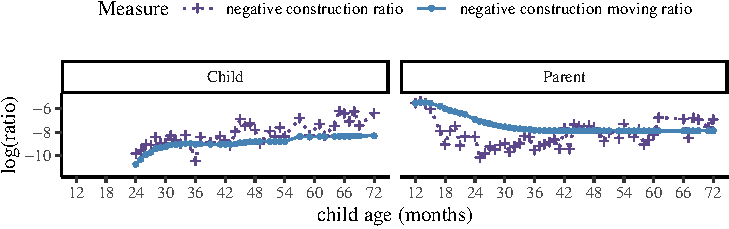
\includegraphics{figs/prohibition-1} \end{center}

\end{CodeChunk}
\caption[This image spans both columns]{Prohibition.}\label{fig:prohibition}
\end{figure*}

\begin{figure*}[h]

\begin{CodeChunk}


\begin{center}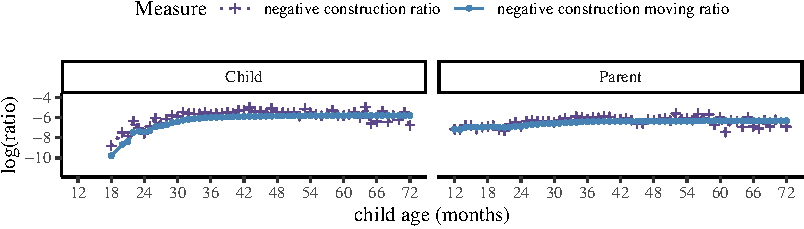
\includegraphics{figs/inability-1} \end{center}

\end{CodeChunk}
\caption[This image spans both columns]{Inability.}\label{fig:inability}
\end{figure*}

\begin{figure*}[h!]

\begin{CodeChunk}


\begin{center}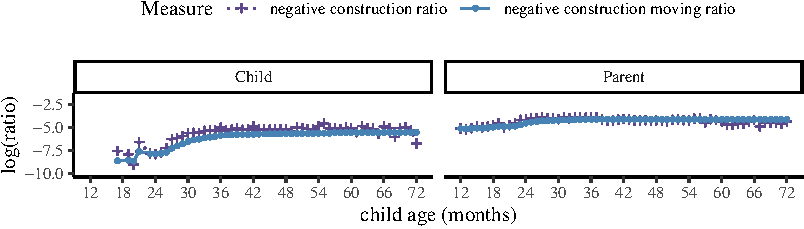
\includegraphics{figs/learning-1} \end{center}

\end{CodeChunk}
\caption[This image spans both columns]{Labeling.}\label{fig:labeling}
\end{figure*}

\hypertarget{inability}{%
\subsubsection{Inability}\label{inability}}

For the function of inability, we analyzed instances where the negative
morphemes co-occur with the auxiliary \emph{can} (\emph{can} and
\emph{could}; e.g.~(8)) and both of them modify the head verbs of the
utterances. Again, we filtered out cases where the head verbs are the
focus for other functions. Cases without a subject (e.g.~\emph{can't
play}) or where the subject is not \emph{I} (e.g.~\emph{you can't do
that}) could yield ambiguous readings when not taking a larger discourse
context into account; they could be a rhetorical question or also
express the concept of prohibition. Therefore to potentially avoid less
ambiguity, we restricted our analyses only to cases with a subject
\emph{I}. This led to 6,369 negative utterances (child: 3,237; parent:
3,132).

~ (8) \emph{I can't see}

As shown in Figure 4, the developmental trajectory of inability is
similar to that for rejection; negation is being applied more and more
regularly between 19-36 months. By contrast, the pattern for inability
is different from those of non-existence and prohibition in at least the
settings that we investigated. It seems that the production trajectories
of the latter two both are becoming more regular at a later age (27 and
24 months, respectively), an observation different from the original
argument by Choi (1988), which proposes vice versa.

\hypertarget{labeling}{%
\subsubsection{Labeling}\label{labeling}}

To capture the function of labeling, we concentrated on cases where
negative morphemes are adopted to indicate the identity (e.g.~(9)),
and/or characteristics (e.g.~(10)) of a predicative nominal. In
addition, we also included instances where the negative morphemes are
used to modify a predicative adjective (e.g.~(11)). Following these
criteria, utterances where the negative morpheme is modifying a nominal
or adjectival predicate of a copula verb were extracted. None of the
utterances contained expletives (\emph{there is no book}) to distinguish
from non-existence. This yielded in a total of 32,474 negative
utterances (Child: 4,180; Parent: 28,294).

~ (9) \emph{that's not a farmer}

~ (10) \emph{I'm not a heavy baby Mum}

~ (11) \emph{It's no good}

Based on Figure 5, the developmental pattern of for labeling is
comparable to non-existence and prohibition; children are increasing
their use of the negative morphemes around the age range of of 22-36
months.

\hypertarget{epistemic-negation}{%
\subsubsection{Epistemic negation}\label{epistemic-negation}}

The function of epistemic negation was originally discussed by Choi
(1988). Although there has been no proposal for negation originating in
children's understanding of their own or others' epistemic/mental
states, previous studies have reported many instances where the negative
morphemes are combined with mental state verbs such as \emph{know},
\emph{think}, and \emph{remember} in child speech. Here we focused on
these three verbs and analyzed utterances that articulate the concept of
unknowing (e.g.~(12)) or uncertainty (e.g.~(13)). The verbs in these
cases are modified by the negative morphemes directly or by the
combination of negation with auxiliaries. By these search criteria,
instances where the speaker inquires about/describes the negative
epistemic state of another speaker (e.g.~(14)) were also selected,
leading to 21,844 negative utterances in total (child: 4,074; parent:
17,770).

~ (12) \emph{I not know} / \emph{I didn't remember}

~ (13) \emph{I don't think so}

~ (14) \emph{don't you remember} / \emph{She doesn't know this}

\begin{figure*}[h!]

\begin{CodeChunk}


\begin{center}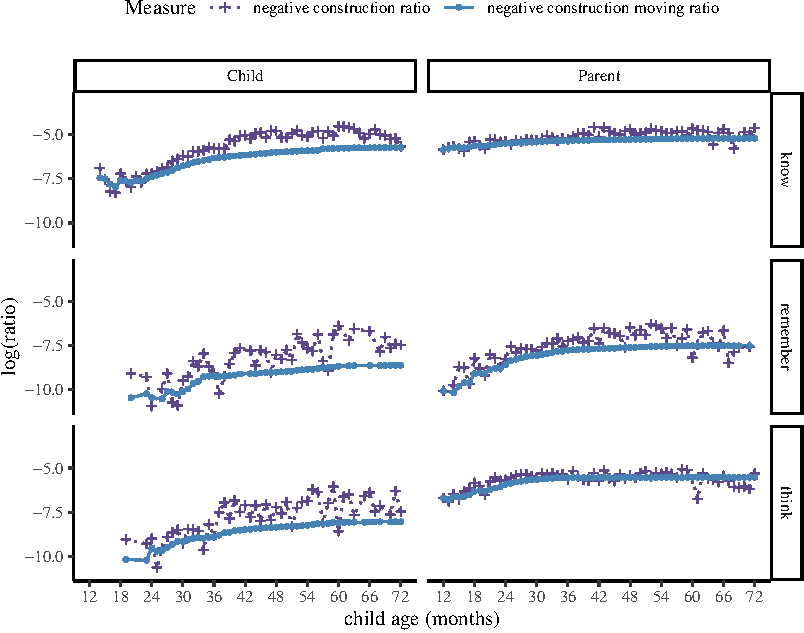
\includegraphics{figs/epistemic-1} \end{center}

\end{CodeChunk}
\caption[This image spans both columns]{Epistemic negation.}\label{fig:epistemic}
\end{figure*}

\begin{figure*}[h!]

\begin{CodeChunk}


\begin{center}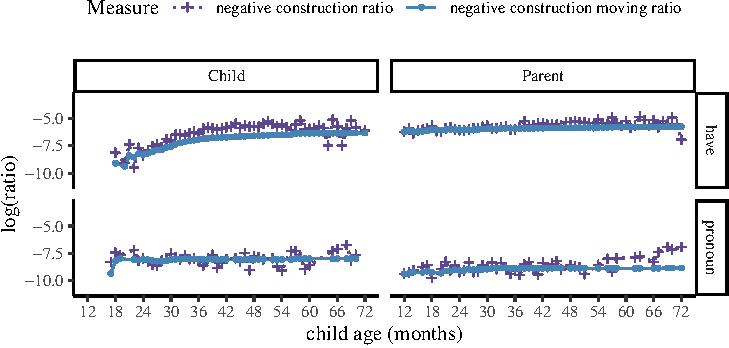
\includegraphics{figs/possession-1} \end{center}

\end{CodeChunk}
\caption[This image spans both columns]{Possession.}\label{fig:possession}
\end{figure*}

\begin{figure*}[h!]

\begin{CodeChunk}


\begin{center}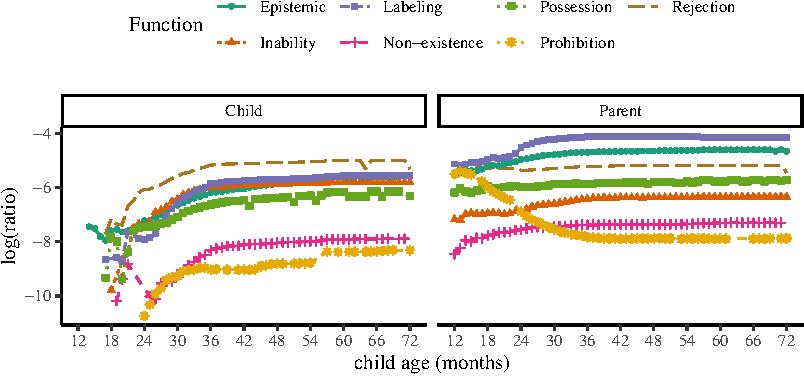
\includegraphics{figs/all-1} \end{center}

\end{CodeChunk}

\caption[This image spans both columns]{All functions; ratio measured plotted here are moving ratios.}\label{fig:all}
\end{figure*}

Based on the data analyzed here (Figure 6), comparing the developmental
trajectories of labeling with the three head verbs in child speech, the
production of negative utterances headed by \emph{know} are becoming
more regular at an earlier age (17-18 months) compared to that of
\emph{remember} (\textasciitilde19 months) or \emph{think}
(\textasciitilde20 months). Overall the production moving ratio of
utterances with \emph{know} is comparatively the highest.

\hypertarget{possession}{%
\subsubsection{Possession}\label{possession}}

The last function that we investigated includes negative utterances that
denote possession. Specifically, we selected cases where the negative
morphemes are combined with auxiliary verbs to modify a head verb with
the lemma form \emph{have} (e.g.~(15)). We also included instances that
are individual noun phrases, where the heads of the noun phrases are
possessive pronouns modified by negative morphemes (e.g.~(16)).
Therefore cases in which the syntactic head of the negative morphemes is
a predicate of a copula verb (e.g.~\emph{this is not mine}) were
excluded to separate from the function of labeling. The number of
negative utterances that were subjected to analysis for this function is
8,187 (child: 2,331; parent: 5,856).

~ (15) \emph{I don't have it}

~ (16) \emph{not mine}

Given Figure 7, the developmental trajectory for possession in child
speech appears to have notable differences depending on what the
negative morphemes are modifying. When their syntactic head is
\emph{have}, the pattern is comparable to the functions such as
rejection and labeling, where children are increasing their combination
of negative morphemes from 19 to 36 months. However, the production
moving ratio for utterances headed by possessive pronouns seems to be
relatively stable across different ages of the children.

\hypertarget{discussion}{%
\section{Discussion}\label{discussion}}

With large-scale corpora of child-parent interactions as well as
automatic annotations, we presented analyses of negative utterances that
express the communicative functions of rejection, non-existence,
prohibition, inability, labeling, epistemic states and possession.
Taking an overall look at the developmental trajectories of all
functions combined shown in Figure 8, it appears that for most of these
communicative functions, the usage of negation is gradually increasing
between the age range of 24-36 months, and stays regular afterwards.

It is important to note that similar to prior studies, our conclusions
are limited to children's production. While it is possible that patterns
in children's production reflect their comprehension and semantic
development overall, this is not guaranteed. Systematic experiments
testing children's comprehension of negative utterances with different
communicative functions are necessary to understand the origin of
negation more thoroughly. And the data presented in our experiments
could be useful stimuli for experiments as such.

For future work, we would like to explore several directions. First, one
limitation of our work here is that to more thoroughly analyze and
potentially model the developmental trajectories of child production,
certain production-specific factors (e.g.~length of utterance, ease of
pronunciation) should be taken into account as well, which we plan to
incorporate in future work. In addition, we aim to investigate the
production trajectory of positive counterparts to our negative
structures (e.g.~\emph{I know} for \emph{I don't know}). This would
allow us to compare the production of positive and negative
constructions and further control for the production trajectory of
specific constructions regardless of whether negation is present.

To validate the findings here furthermore, we also intend to examine
negative utterances produced by individual children with our methods and
analyses. Lastly, our experiments thus far have concentrated on
syntactic structures at the utterance level, therefore cases where
negations are used as discourse markers to respond to previous
utterance(s) were excluded. However, these instances also have important
semantic and conceptual roles in the communication between children and
parents (e.g.~Parent: \emph{do you want some bread?}; Child: \emph{no no
no}). Thus inclusions of negative structures at the discourse level
would be able to paint a more clear picture about the development of
negation.

\hypertarget{references}{%
\section{References}\label{references}}

\setlength{\parindent}{-0.1in} 
\setlength{\leftskip}{0.125in}

\noindent

\hypertarget{refs}{}
\leavevmode\hypertarget{ref-diaparser}{}%
Attardi, G., Sartiano, D., \& Yu, Z. (n.d.). DiaParser attentive
dependency parser. \emph{Submitted for Publication}.

\leavevmode\hypertarget{ref-bloom1970language}{}%
Bloom, L. M. (1970). \emph{Language development: Form and function in
emerging grammars} (PhD thesis). Columbia University.

\leavevmode\hypertarget{ref-cameron2007part}{}%
Cameron-Faulkner, T., Lieven, E., \& Theakston, A. (2007). What part of
no do children not understand? A usage-based account of multiword
negation. \emph{Journal of Child Language}, \emph{34}(2), 251.

\leavevmode\hypertarget{ref-choi1988semantic}{}%
Choi, S. (1988). The semantic development of negation: A
cross-linguistic longitudinal study. \emph{Journal of Child Language},
\emph{15}(3), 517--531.

\leavevmode\hypertarget{ref-clark2010adult}{}%
Clark, E. V. (2010). Adult offer, word-class, and child uptake in early
lexical acquisition. \emph{First Language}, \emph{30}(3-4), 250--269.

\leavevmode\hypertarget{ref-darwin1872expression}{}%
Darwin, C. (1872). \emph{The expression of the emotions in man and
animals}. John Murray.

\leavevmode\hypertarget{ref-demuth2006word}{}%
Demuth, K., Culbertson, J., \& Alter, J. (2006). Word-minimality,
epenthesis and coda licensing in the early acquisition of English.
\emph{Language and Speech}, \emph{49}(2), 137--173.

\leavevmode\hypertarget{ref-macwhinney2000childes}{}%
MacWhinney, B. (2000). \emph{The childes project: Tools for analyzing
talk. Transcription format and programs} (Vol. 1). Psychology Press.

\leavevmode\hypertarget{ref-nordmeyer2018individual}{}%
Nordmeyer, A., \& Frank, M. C. (2018). Individual variation in
children's early production of negation. In \emph{CogSci}.

\leavevmode\hypertarget{ref-pea1978}{}%
Pea, R. (1978). \emph{The development of negation in early child
language} (PhD thesis). University of Oxford.

\leavevmode\hypertarget{ref-sagae2010morphosyntactic}{}%
Sagae, K., Davis, E., Lavie, A., MacWhinney, B., \& Wintner, S. (2010).
Morphosyntactic annotation of childes transcripts. \emph{Journal of
Child Language}, \emph{37}(3), 705--729.

\leavevmode\hypertarget{ref-sanchez2019childes}{}%
Sanchez, A., Meylan, S. C., Braginsky, M., MacDonald, K. E., Yurovsky,
D., \& Frank, M. C. (2019). Childes-db: A flexible and reproducible
interface to the child language data exchange system. \emph{Behavior
Research Methods}, \emph{51}(4), 1928--1941.

\leavevmode\hypertarget{ref-dg}{}%
Tesnière, L. (1959). \emph{Éléments de syntaxe structurale}. Paris:
Klincksieck.

\leavevmode\hypertarget{ref-de1979form}{}%
Villiers, P. A. de, \& Villiers, J. G. de. (1979). Form and function in
the development of sentence negation. \emph{Papers and Reports on Child
Language Development}, \emph{17}, 57--64.

\leavevmode\hypertarget{ref-wei2006time}{}%
Wei, W. W. (2006). Time series analysis. In \emph{The oxford handbook of
quantitative methods in psychology: Vol. 2}.

\bibliographystyle{apacite}


\end{document}
